\cleardoublepage
\chapter{Solução} \label{capituloSolucoes}

Neste capítulo iremos explorar a solução encontrada para os vários desafios e necessidades encontradas ao longo desta dissertação.
\vspace{-4mm}
\section{Autenticação local}
\vspace{-4mm}
\subsection{Especificação} \label{especificacaoAuthLocal}
\vspace{-3mm}
De modo a satisfazer as necessidades da autenticação local de utilizadores, através de username e password, foi decidida a implementação de uma base de dados em \emph{MongoDB}.

A criação de um utilizador na plataforma \gls{clav} obriga ao preenchimento dos seguintes dados:

\begin{enumerate}
    \item \textbf{Nome}
    
        Qualquer combinação de números e letras.
    \item \textbf{Email}
    
        Considera-se um email válido qualquer combinação de letras e números, seguida de um "@" com terminação em "." seguido de letras.
    \item \textbf{Nível de utilizador}
    
        Durante a fase de registo é obrigatória a seleção do nível de utilizador do mesmo, sendo esta utilizada para verificação de nível de acesso dentro da plataforma \gls{clav}.
    \begin{enumerate}
        \item Administrador de Perfil Tecnológico
        \item Administrador de Perfil Funcional
        \item Utilizador Validador
        \item Utilizador Avançado
        \item Utilizador Decisor (AD)
        \item Utilizador Decisor
        \item Utilizador Simples
        \item Representante Entidade
    \end{enumerate}
    \item \textbf{Entidade}
    
        A escolha de uma entidade ao qual o utilizador pertence é de caratér obrigatório, não sendo permitido o registo sem a mesma ser selecionada. Para tal efeito, é carregada a lista de entidades já registadas no sistema das quais o utilizador escolherá uma.
        
    \item \textbf{Password}
    
        Qualquer combinação de números e letras.
\end{enumerate}
\vspace{-1mm}
Além da obrigatoriedade dos dados prévios, foi também decidido que todos os dados relativos aos utilizadores iriam ser guardados numa coleção MongoDB com o nome "\emph{users}".

\vspace{-6mm}
\subsection{Workflow da autenticação}
\vspace{-9mm}
\begin{figure}[ht!]
    \centering
    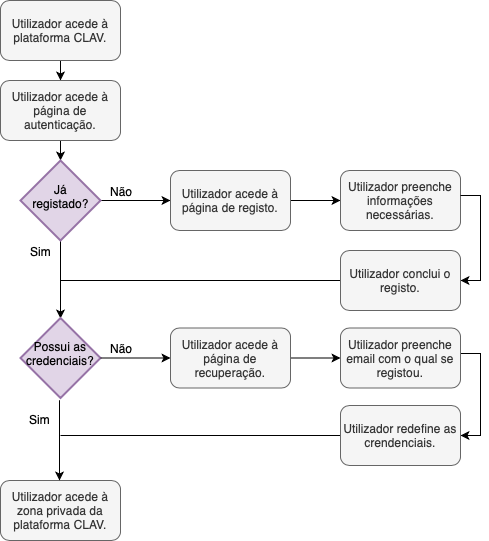
\includegraphics[width=0.65\textwidth]{img/diagramas/authlocal/AuthLocal.png}
    \caption{Workflow da autenticação local.}
    \label{fig:flow_authlocal}
\end{figure}

\cleardoublepage
\section{Autenticação através de Cartão de Cidadão}
\subsection{Especificação}

A autenticação através de Cartão de Cidadão é baseada na autenticação local, havendo distinção entre os utilizadores registados via username e password, e aqueles registados através de Cartão de Cidadão.

\begin{enumerate}
    \item \textbf{Nome}
    
        Qualquer combinação de números e letras.
    \item \textbf{Email}
    
        Considera-se um email válido qualquer combinação de letras e números, seguida de um "@" com terminação em "." seguido de letras.
    \item \textbf{Nível de utilizador}
    
        Durante a fase de registo é obrigatória a seleção do nível de utilizador do mesmo, sendo esta utilizada para verificação de nível de acesso dentro da plataforma \gls{clav}.
    \begin{enumerate}
        \item Administrador de Perfil Tecnológico
        \item Administrador de Perfil Funcional
        \item Utilizador Validador
        \item Utilizador Avançado
        \item Utilizador Decisor (AD)
        \item Utilizador Decisor
        \item Utilizador Simples
        \item Representante Entidade
    \end{enumerate}
    \item \textbf{Entidade}
    
        A escolha de uma entidade ao qual o utilizador pertence é de caratér obrigatório, não sendo permitido o registo sem a mesma ser selecionada.
\end{enumerate}

\cleardoublepage
\subsection{Workflow da autenticação}

\begin{figure}[h!]
    \centering
    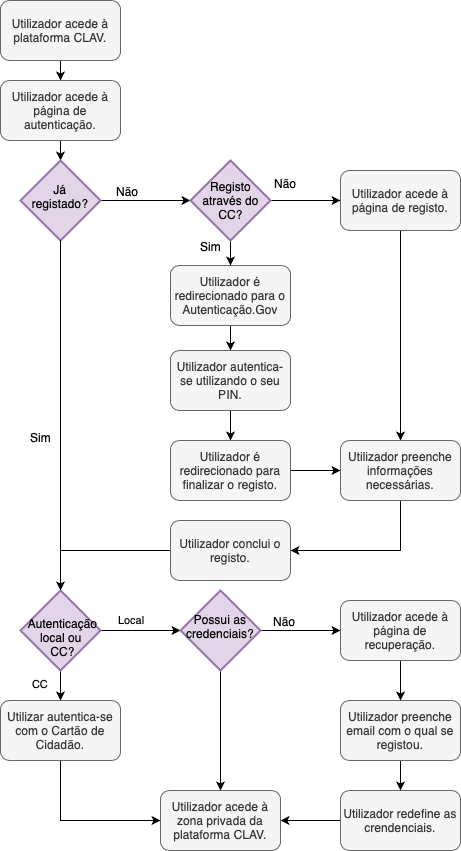
\includegraphics[width=0.695\textwidth]{img/diagramas/authCC/AuthCC.png}
    \caption{Workflow da autenticação através de Cartão de Cidadão.}
    \label{fig:flow_authCC}
\end{figure}

\cleardoublepage
\section{Proteção da API de dados} \label{protecaoAPI}

\subsection{Especificação}

De modo a fornecer uma camada de proteção à \gls{api} de dados, é necessário identificar e autenticar os pedidos que a ela chegam.

Para tal, a solução encontrada foi a implementação de duas funções de middleware responsáveis pela seguinte função:

\begin{enumerate}
    \item \textbf{Verificação da origem do pedido}
    
    Função de middleware cujo funcionamento é baseado em tokens \gls{jwt}. Esta função é executada sempre que há um pedido à \gls{api} e verifica se o pedido obedece aos seguintes critérios:

    \begin{enumerate}
        \item \textbf{Presença do token}
        
        Todo e qualquer pedido à \gls{api} de dados da plataforma \gls{clav}, seja um \emph{GET}, \emph{POST}, entre outros, tem de ser enviado com um token baseado em \gls{jwt}.
        
        \item \textbf{Validade do token}
        
        Após receção do token, este irá ser descodificado e irá ocorrer a verificação da validade do mesmo, ou seja, se o token é válido e contem o identificador do utilizador que fez o pedido à API.
    \end{enumerate}
    
    \item \textbf{Verificação do nível de acesso}
    
    Caso o token seja válido e de facto contem o identificador do utilizador, é verificado o nível de acesso do mesmo. Caso este esteja a tentar aceder a funções da \gls{api} que necessitam de um nível superior ao fornecido, o pedido é negado, caso contrário é permitido o acesso à informação pedida. 
\end{enumerate}

\cleardoublepage
\subsection{Workflow da autenticação}

\begin{figure}[h!]
    \centering
    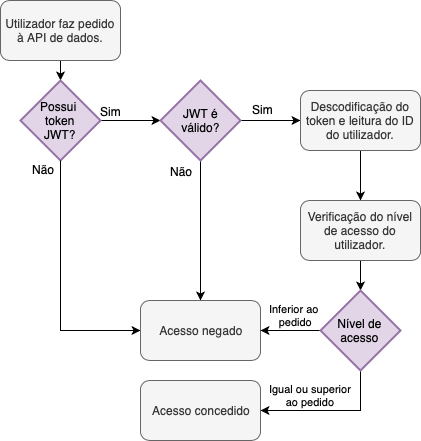
\includegraphics[width=0.8\textwidth]{img/diagramas/authAPI/AuthAPI.png}
    \caption{Workflow da autenticação de pedidos à API de dados.}
    \label{fig:flow_authCC}
\end{figure}

\cleardoublepage
\section{Gestão de utilizadores} \label{gestaoUtilizadoresSolucao}

\subsection{Especificação}
De modo a fornecer uma solução para a gestão de utilizadores, foi sugerida a criação e implementação de uma página que correspondesse a um painel de gestão de utilizadores.

Este painel de gestão terá de suportar as seguintes funcionalidades:

\begin{enumerate}
    \item Listagem de todos os utilizadores registados na plataforma \gls{clav}.
    \item Filtragem de utilizadores através de campo de pesquisa.
    \item Ordenação de utilizadores através dos seguintes parâmetros:
    \begin{enumerate}
        \item Nome.
        \item Entidade.
        \item Email.
        \item Nível de utilizador.
    \end{enumerate}
\end{enumerate}

Além das funcionalidades previamente descritas, este painel de gestão terá de permitir a edição dos utilizadores em causa, permitindo alterar os parâmetros previamente listados, bem como suportar a desactivação de um utilizador, sendo a este interdito o acesso à plataforma \gls{clav} enquanto não for desbloqueado.

\cleardoublepage
\subsection{Workflow da edição de um utilizador}

\begin{figure}[h!]
    \centering
    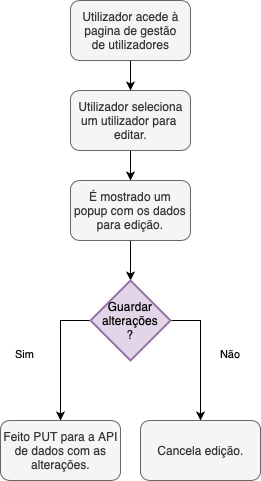
\includegraphics[width=0.5\textwidth]{img/diagramas/gestaometrica/Edicao.png}
    \caption{Workflow da edição de um utilizador na plataforma \gls{clav}.}
    \label{fig:flow_Edicao}
\end{figure}

\cleardoublepage
\section{Métrica da plataforma} \label{solucaoMetrica}
\vspace{-4mm}
\subsection{Especificação}
\vspace{-4mm}
Além das medidas especificadas na secção \ref{protecaoAPI}, foi sugerida a criação de uma página capaz de identificar a quantidade de pedidos processados pela plataforma \gls{clav}. Para tal, é necessário distinguir entre os possíveis tipo de pedidos existentes na API de dados: 
\vspace{-3mm}
\begin{itemize}
    \item \textbf{GET}.
    \vspace{-1.5mm}
    \item \textbf{POST}.
    \vspace{-1.5mm}
    \item \textbf{PUT}.
    \vspace{-1.5mm}
    \item \textbf{DELETE}.
\end{itemize}

\vspace{-1mm}
Além de ser guardado em base de dados o tipo de pedido feito, irá ser guardado a API de qual o pedido originou, quer seja ela a API dos utilizadores, das entidades, classes, etc, de forma a ser possível visualizar graficamente qual é a API mais utilizada.

Este recolher de dados permite também evitar utilizações indevidas da API de dados pública. Por exemplo, um elevado acesso à API pode levar a uma resposta extremamente demorada por parte do servidor, bem como o "crash" total da aplicação devido a esgotamento de recursos. Estes ataques são extremamente comuns e devido à implementação de métrica, é possível prevenir os mesmos de modo a eliminar esse risco.

\vspace{-6mm}
\subsection{Workflow da incrementação da métrica na plataforma}
\vspace{-10mm}
\begin{figure}[ht!]
    \centering
    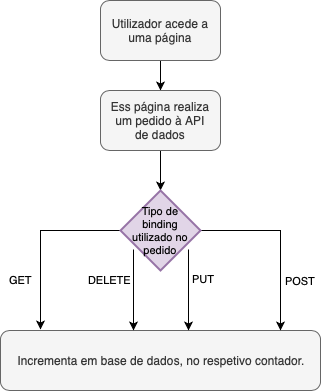
\includegraphics[width=0.41\textwidth]{img/diagramas/gestaometrica/Metrica.png}
    \caption{Workflow da incrementação de métrica na plataforma \gls{clav}.}
    \label{fig:flow_Metrica}
\end{figure}

\cleardoublepage
\section{Síntese}

Uma das principais necessidades desta dissertação recaiu na documentação de todo o processo de desenvolvimento. 

Esta documentação tem como objetivo explicar de forma explícita e com alto detalhe toda a arquitetura aplicacional implementada no projeto \gls{clav}, sendo que para tal foram utilizados diagramas de fluxo que explicam de forma clara esta mesma solução.

O principal foco deste capítulo baseou-se na autenticação de utilizadores, quer por autenticação local, bem como por Cartão de Cidadão através do Autenticação.Gov e da protecção da API de dados disponibilizada ao público.

No seguinte capítulo irá ser descrita a implementação utilizada nas vertentes da plataforma \gls{clav}.